% c4-treeclock-v.tex

\documentclass{standalone}
% newcommands.tex

\newcommand{\enq}{\texttt{enq}}
\newcommand{\deq}{\texttt{deq}}
\newcommand{\pput}{\texttt{PUT}}
\newcommand{\get}{\texttt{GET}}
\newcommand{\vs}{\texttt{vis}}
\newcommand{\so}{\texttt{so}}
\newcommand{\arb}{\texttt{ar}}
\newcommand{\rf}{\texttt{rf}}

% example
\newcommand{\po}[2]{\draw [->, thick] (#1) to node[above] {\Large{\so}} (#2);}
\newcommand{\pva}[2]{\draw [->, thick] (#1) to node[above] {$\Large{\so},\Large{\vs},\Large{\arb}$} (#2);}
\newcommand{\pbva}[2]{\draw [->, thick] (#1) to node[above] {$\Large{\so}$} node[below] {$\Large{\vs},\Large{\arb}$} (#2);}
\newcommand{\pv}[2]{\draw [->, thick] (#1) to node[above] {\Large{\so}} node[below] {\Large{\vs}} (#2);}
\newcommand{\evis}[2]{\draw [->, thick] (#1) to node[above, sloped, near end] {\Large{\vs}} (#2);}
\newcommand{\mvis}[2]{\draw [->, thick] (#1) to node[above, sloped] {\Large{\vs}} (#2);}
\newcommand{\ar}[2]{\draw [->, thick, allow upside down] (#1) to node[above, sloped] {\Large{\arb}} (#2);}
\newcommand{\va}[2]{\draw [->, thick, allow upside down] (#1) to node[above, sloped] {$\Large{\vs},\Large{\arb}$} (#2);}
\newcommand{\vab}[2]{\draw [->, thick, allow upside down] (#1) to node[below, sloped, near end] {$\Large{\vs},\Large{\arb}$} (#2);}
\newcommand{\vae}[2]{\draw [->, thick, allow upside down] (#1) to node[above, sloped, near end] {$\Large{\vs},\Large{\arb}$} (#2);}
\newcommand{\vas}[2]{\draw [->, thick, allow upside down] (#1) to node[sloped, near start, above] {$\Large{\vs},\Large{\arb}$} (#2);}

% serialization
\newcommand{\scc}[2]{\draw [->, very thick] (#1) to (#2);}
\newcommand{\rva}[2]{\draw [->, thick, allow upside down] (#1) to node[above, sloped] {$\Large{\rf},\Large{\vs},\Large{\arb}$} (#2);}
\newcommand{\rvb}[2]{\draw [->, thick, allow upside down] (#1) to node[below, sloped] {$\Large{\rf},\Large{\vs},\Large{\arb}$} (#2);}


\usepackage{tikz}
\usetikzlibrary{shapes, positioning, arrows.meta, decorations.pathmorphing}

\begin{document}
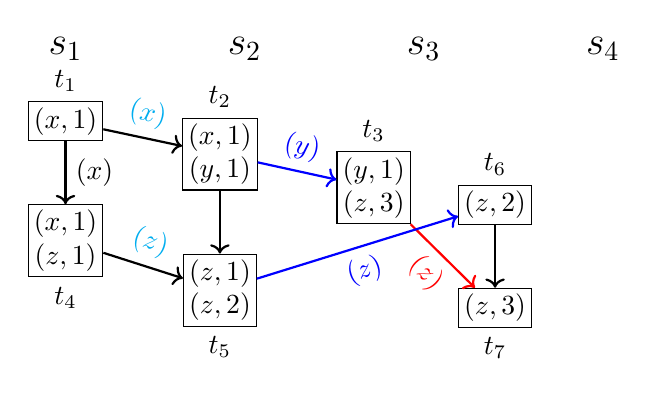
\begin{tikzpicture}[
  so/.style = {->, thick},
  wr/.style = {->, thick},
  co/.style = {->, thick},
  vo/.style = {->, thick},
  txn/.style = {draw, inner sep = 2pt}]

  % t1: W(x, 1)
  \node[txn, label = above : $t_{1}$]
		(t1) {$\writeevent(x, 1)$};
  % t4: R(x, 1) W(z, 1)
  \node[txn, below = 0.80cm of t1, label = below : $t_{4}$, align = center]
    (t4) {$\readevent(x, 1)$\\$\writeevent(z, 1)$};

  % t2: R(x, 1) W(y, 1)
  \node[txn, below right = -0.30cm and 1.00cm of t1,
    label = above : $t_{2}$, align = center]
    (t2) {$\readevent(x, 1)$\\$\writeevent(y, 1)$};
	% t5: R(z, 1) W(z, 2)
  \node[txn, below = 0.80cm of t2, label = below : $t_{5}$, align = center]
    (t5) {$\readevent(z, 1)$\\$\writeevent(z, 2)$};

  % t3: R(y, 1) W(z, 3)
  \node[txn, below right = -0.50cm and 1.00cm of t2,
    label = above : $t_{3}$, align = center]
    (t3) {$\readevent(y, 1)$\\$\writeevent(z, 3)$};

	% t6: R(z, 2)
  \node[txn, below right = -0.50cm and 0.60cm of t3,
    label = above : $t_{6}$]
    (t6) {$\readevent(z, 2)$};
	% t7: R(z, 3)
  \node[txn, below = 0.80cm of t6, label = below : $t_{7}$]
    (t7) {$\readevent(z, 3)$};

	% session s1
	\node[above = 0.40cm of t1, font = \Large] (s1) {$s_{1}$};
	\node[right = 1.60cm of s1, font = \Large] (s2) {$s_{2}$};
	\node[right = 1.60cm of s2, font = \Large] (s3) {$s_{3}$};
	\node[right = 1.60cm of s3, font = \Large] (s4) {$s_{4}$};

  % t1-SO-t4
  \draw[so] (t1) to node[left]{$\SO$} node[right]{$\WR(x)$} (t4);
	% t2-SO-t5
  \draw[so] (t2) to node[right]{$\SO$} (t5);
	% t6-SO-t7
  \draw[so] (t6) to node[right]{$\SO$} (t7);

	% t1-t2-t3-t7
	\draw[wr] (t1) to node[sloped, above, cyan] {$\WR(x)$} (t2);
	\draw[wr, blue] (t2) to node[sloped, above] {$\WR(y)$} (t3);
	\draw[wr, red] (t3) to node[sloped, below] {$\WR(z)$} (t7);

	% t4-t5-t6
	\draw[wr] (t4) to node[sloped, above, cyan] {$\WR(z)$} (t5);
	\draw[wr, blue] (t5) to node[sloped, below] {$\WR(z)$} (t6);
\end{tikzpicture}
\end{document}